% -*- latex -*-
%-----------------------------------------------------------------------
%;  Copyright (C) 2010
%;  Associated Universities, Inc. Washington DC, USA.
%;
%;  This program is free software; you can redistribute it and/or
%;  modify it under the terms of the GNU General Public License as
%;  published by the Free Software Foundation; either version 2 of
%;  the License, or (at your option) any later version.
%;
%;  This program is distributed in the hope that it will be useful,
%;  but WITHOUT ANY WARRANTY; without even the implied warranty of
%;  MERCHANTABILITY or FITNESS FOR A PARTICULAR PURPOSE.  See the
%;  GNU General Public License for more details.
%;
%;  You should have received a copy of the GNU General Public
%;  License along with this program; if not, write to the Free
%;  Software Foundation, Inc., 675 Massachusetts Ave, Cambridge,
%;  MA 02139, USA.
%;
%;  Correspondence concerning AIPS should be addressed as follows:
%;          Internet email: aipsmail@nrao.edu.
%;          Postal address: AIPS Project Office
%;                          National Radio Astronomy Observatory
%;                          520 Edgemont Road
%;                          Charlottesville, VA 22903-2475 USA
%-----------------------------------------------------------------------
%Body of final AIPSletter for 31 December 2010

\documentclass[twoside]{article}
\usepackage{graphics}

\newcommand{\AIPRELEASE}{December 31, 2010}
\newcommand{\AIPVOLUME}{Volume XXX}
\newcommand{\AIPNUMBER}{Number 2}
\newcommand{\RELEASENAME}{{\tt 31DEC10}}
\newcommand{\OLDNAME}{{\tt 31DEC09}}
\newcommand{\NEWNAME}{{\tt 31DEC11}}

%macros and title page format for the \AIPS\ letter.
\input LET98.MAC

\newcommand{\MYSpace}{-11pt}

\normalstyle

\section{General developments in \AIPS}

\subsection{Current and future releases}

We have formal \AIPS\ releases on an annual basis.  We recommend a
full binary installation method for both the frozen and development
versions for MacIntosh OS/X (PPC and Intel chips), Solaris, and Linux
(32- and 64-bit) systems, but all architectures can do a full
installation from the source files.  If you develop \AIPS\ code
locally, you will need to do a source-level installation.  The current
release is called \RELEASENAME\ and is now ``frozen.''  If you took a
development copy of this version at some earlier date, you should use
the ``Midnight Job'' (MNJ) to bring it up to date.  You need to run a
MNJ only once in 2011 to convert your copy of \RELEASENAME\ into the
frozen version.  When patches to \RELEASENAME\ are announced, you may
apply them with the MNJ\@.  This \Aipsletter\ is intended to advise
you of corrections and improvements in this release.

We have begun a new version, called \NEWNAME, which is now under
development by the \AIPS\ Group.  You may fetch and install a complete
copy of this version at any time.  Having fetched \NEWNAME, you may
update your installation whenever you want by running the MNJ\@.  This
uses cvs, rsync, and/or transaction files to copy and compile the code
selectively based on the code changes and compilations we have done.
We expect users to take their source-only or binary version of
\NEWNAME\ \AIPS\ over the Internet (via \emph{anonymous} ftp).  Both
versions require you to copy the installation procedure {\tt
install.pl} via {\tt ftp}; the source-only version also requires you
to ftp the 108-Mbyte {\tt \NEWNAME.tar.gz} compressed tar file.  Linux
sites will almost certainly have {\tt cvs} installed; other sites may
have installed it along with other GNU tools.  Secondary MNJs will
still be possible using {\tt ssh} or {\tt rcp} or NFS as with previous
releases.  We have found that {\tt cvs} works very well, although it
has one quirk.  If a site modifies a file locally but in an
\AIPS-standard directory, {\tt cvs} will detect the modification and
attempt to reconcile the local version with the NRAO-supplied version.
This usually produces a file that will not compile or run as intended.

\AIPS\ is now copyright \copyright\ 1995 through 2010 by Associated
Universities, Inc., NRAO's parent corporation, but may be made freely
available under the terms of the Free Software Foundation's General
Public License (GPL)\@.  This means that User Agreements are no longer
required, that \AIPS\ may be obtained via anonymous ftp without
contacting NRAO, and that the software may be redistributed (and/or
modified), under certain conditions.  The full text of the GPL can be
found in the \texttt{15JUL95} \Aipsletter\ and is included with every
distribution in file {\tt \$AIPS\_ROOT/{\it release-name}/COPYING}\@.
\vfill\eject

\subsection{Installing a new version}

If compiling locally, new releases must be installed from the tar ball
for that release.  If using the binary installation, a full new
installation must also be done with {\tt rsync}.  The {\tt cvs} system
requires this.  When installing a new \AIPS\ release in a system that
already has a previous release, we recommend that {\tt install.pl} be
used and that the previous release be left in place, at least until
the new installation has been seen to work.  If you do this, then you
will not have to re-edit the disk, printer, and tape lists and can
simply skip all those pages in the {\tt install.pl} menus.  The old
{\tt \$HOME/.AIPSRC} file may be left in place, but it will need to be
edited.  The lines giving the {\tt DOWNLOADED} and {\tt UNPACKED}
parameters should be cleared and the {\tt CCOMOPT} line should be
changed to point to the current release rather than the previous one
--- the {\tt -I} parameter really should be {\tt -I\$INC} but it gets
its full path name instead.  This forces a re-edit with each release.
If you have made special versions of {\tt UPDCONFIG} and {\tt
do\_daily.{\it host}}, you should preserve them under new names and
restore them after the install.  If you have an odd set of \AIPS\
versions, the {\tt \$AIPS\_ROOT/AIPSPATH.*SH} files may need to be
edited after the install to set the desired versions.

For Linux, Solaris Ultra, and MacIntosh systems, a binary installation
could be available from DVD, supported by {\tt install.pl}.
Alternatively, the frozen version may be installed with the binary
installation method now present in {\tt install.pl}.  The ftp site for
downloading files directly has been eliminated.

\section{\AIPS\ Distribution}

From the NRAO system logs, we count apparent MNJ accesses, downloads
of the tar balls, and {\tt rsync} accesses by unique IP address.
Since DSL and some university and other connections may be assigned
different IP addresses at different times, this will be a bit of an
over-estimate of actual sites.  However, a single IP address is often
used to provide \AIPS\ to a number of computers, so these numbers are
at the same time an under-estimate of the number of computers running
current versions of \AIPS\@.  In 2010, a total of 307 different IP
addresses downloaded the frozen form of \OLDNAME\ and 1228 IP
addresses downloaded \RELEASENAME\ in tarball or binary form.  Fully
1914 IP addresses accessed the NRAO cvs master.  Each of these has at
least installed some version of \AIPS\ and 535 appear to have run the
MNJ at least occasionally.  The total number of unique IP addresses in
these three lists was 2416.  477 sites accessed \OLDNAME\ in binary
form, while 1203 sites used the binary form of \RELEASENAME\@.  The
attached figure shows the cumulative number of unique sites, cvs
access sites, tar-ball/binary download sites and binary access sites
known to us as a function of week in 2009.  These numbers are
remarkably similar to those of 2009.

\centerline{\resizebox{4.8in}{!}{\includegraphics{FIG/PLOTIT10b.PS}}}

\vfill\eject

\section{Preview of coming attractions}

The \NEWNAME\ release already contains a few changes that we decided
were a bit risky or not needed in \RELEASENAME\@.  {\tt CLSMO} and
{\tt SNSMO} have normalization controls, {\tt TVFLG} has a revision of
the next IF option and its image placement, {\tt TYSMO} applies flag
tables to the {\tt TY} or {\tt SY} tables on input, a new task {\tt
REWGT} applies user-specified scaling to data weights, and a number
of tasks will now select on {\tt CALCODE} as well as source name.

\section{Improvements of interest to users in \RELEASENAME}

We expect to continue publishing the \Aipsletter\ every six months
along with the annual releases.  There are a few new tasks released in
the last six months, but the biggest changes have taken place in
existing tasks used now for EVLA calibration.  New tasks include {\tt
  SOUSP} to fit spectral indices from the fluxes in the source table,
{\tt NOIFS} to convert a multi-channel, multi-IF data base into one
with a single IF, {\tt TRUEP} to fits for true instrumental
polarization using data taken with rotated feeds, and {\tt SWAPR} to
swap real and imaginary parts of visibility data which may be needed
due to a bug in the {\tt REBYTE} program.  New verb {\tt TVHELIX}
implements Dave Green's helical coloring scheme said to make perceived
brightness increase monotonically.  The biggest changes in existing
tasks involve implementing EVLA gain calibration from SysPower tables
through {\tt TYSMO} and {\tt TYAPL} and spectral-channel dependent
polarization calibration through {\tt PCAL} and {\tt RLDIF}\@.  In the
first six months of \RELEASENAME\ the new tasks were {\tt UVRFI} to
apply RFI mitigation techniques rather than simple flagging, {\tt
  EVASN} and {\tt EVAUV} to examine the remains after pipeline
reduction to determine how well things went, {\tt REWAY} to estimate
the weight of data from the rms found across spectral channels within
the given polarization and IF, {\tt RSPEC} to determine the spectra of
the rms in a data cube, and {\tt RLDLY} to determine the right-left
delay difference.

Normally, bugs which are created in an \AIPS\ {\tt TST} version and
then fixed in that same version before its release get little or no
discussion in the \Aipsletter\@.  Since a rather large number of sites
now install the {\tt TST} version of \AIPS\ during its development,
this is somewhat of an oversight.  We urge you to run the ``Midnight
Job'' at least once after \RELEASENAME\ is frozen to bring it up to
date and to fix all bugs of this sort.  We urge active sites to use
the MNJ and, when something odd occurs, to examine {\tt CHANGE.DOC}
using the cgi tool available from the \AIPS\ web page under
documentation.  Please do not hesitate to e-mail {\tt daip@nrao.edu}
with any questions or suspicions that there are problems.

\OLDNAME\ contains a change in the format of antenna files.  Previous
releases will not understand the antenna coordinates for arrays that
were traditionally left-handed (VLBI primarily).  The format change
occurs automatically when any \OLDNAME\ or later antenna-file specific
code reads the file, after which older releases will have
difficulties.  {\tt  31DEC04} through \NEWNAME\ use a new numbering
scheme for magnetic tape logical unit numbers that is incompatible
with previous versions.  Thus all tape tasks and the server {\tt
  TPMON} must be from a recent release.  Other than these issues,
\OLDNAME\ is compatible in all major ways with the with the {\tt
  15OCT98} and later releases.  There are significant
incompatibilities with older versions.  Note that the only version
which we patch for major errors is \RELEASENAME; even \OLDNAME\ is no
longer changed.

\subsection{Analysis}

While ordinary spectral index is easily defined, the need for spectral
index curvature forces us into a much more rigorous definition.  That
is now
\begin{eqnarray*}
  R & \equiv & \log ( F / 10^9 ) \\
 \log ( T / T_0 ) & = & a R + b R^2 + c R^3 + \ldots \\
\end{eqnarray*}
where $\log$ is a logarithm base 10, $F$ is the frequency in Hz,
$T_0$ is $T$ at 1 GHz frequency, $a$ is the usual spectral index, and
$b, c, \ldots$ are the spectral index curvature terms.  This change of
definition was implemented directly in {\tt SPIXR} and {\tt UVMOD} and
the component modeling offered by {\tt IMAGR} and {\tt OOSUB}\@.  It
affects the implementation of spectral index in a wide variety of
other tasks to be discussed below.
\vfill\eject

Other ``analysis'' topics include a change to {\tt TRANS} which was
found to be able to get into very unfortunate disk access issues while
row swapping.  It will now take large amounts of dynamic memory and
attempt to avoid these issues.  The recording of actual Clean beam
size as a function of channel begun near the start of this release
cycle meant that image files have more than just Clean Component
({\tt CC}) tables attached.  Clean Gaussian ({\tt CG}) and frequency
({\tt FQ}) tables may also be present.  A large number of tasks were
modified to copy these tables from the input to the output, omitting
the {\tt CC}s in around half of the cases.

\subsection{UV data}

\subsubsection{EVLA data acquisition}

EVLA data are recorded using two types of formats, the ASDM or science
data model which contains a variety of xml files describing the data
set and the BDF or binary data format containing the visibilities.
These are available from the archive but need to be translated in
order to be useful in CASA or in \AIPS\@.  One route to \AIPS\
involves first a translation into CASA measurement sets followed by a
translation into $uv$ FITS format which is then read by {\tt UVLOD} or
{\tt FITLD}\@.  A new route has become available through a software
package called {\tt obit} written by Bill Cotton.  If you have the
data in ASDM/BDF form on your computer and {\tt obit} is installed,
you may run a procedure outside of {\tt AIPS} called {\tt BDF2AIPS}
which will perform the translation directly into \AIPS\ files in your
\AIPS\ data area.  This has two major advantages.  It avoids several
data copy/translation steps and so is significantly faster.  More
importantly however, it also produces several \AIPS\ extension files
not currently available through CASA\@.  Index ({\tt NX}), calibration
({\tt CL}) including opacities and gains, flag ({\tt FG}), calDevice
({\tt CD}) $T_{\rm cal}$ values, and sysPower ({\tt SY}) tables are
among these tables.  {\tt obit} is currently the only route to get the
{\tt SY} data which will be significant in proper calibration of EVLA
data.  Observers not in Socorro should be able --- eventually --- to
get $uv$ FITS files from the archive produced either by the CASA or
the {\tt obit} route.

\subsubsection{EVLA gain calibration}

The EVLA ``WIDAR'' correlator is a very linear device over a wide
range of input power.  Therefore, the correlator will deliver
cross-power spectra without internal normalization by the
autocorrelation ``self'' powers.  To determine the system temperatures
and correct for changes in system gain, it is necessary to switch a
noise tube on and off and to record the total power when it is on and
when it is off.  In the case of the EVLA, the recorded parameters are
$P_{sum} = G(P_{on} + P_{off})$ and $P_{dif} = G(P_{on} - P_{off})$,
where $G$ is the gain following the synchronous detector.  These data
are recorded as a function of IF, polarization, and time for each
antenna in the {\tt SY} table written by the {\tt obit} program {\tt
  BDFIn} invoked from the script {\tt BDF2AIPS}\@.  The system
temperature is given by $T_{cal} \times P_{sum} / P_{dif}$ which may
be used to determine data weights and the square root of the product
of $P_{dif} / T_{cal}$ for the two antennas may be used to correct
cross-power into visibilities.

The {\tt SY} tables have become available in the past six months and a
variety of tools have been extended to manipulate, edit, and apply
them.  {\tt SNPLT} may be used to plot all possible combinations of
the {\tt SY} table parameters.  {\tt EDITA} may be used to edit $uv$
data based on the contents of the {\tt SY} table, while {\tt SNEDT}
may be used to edit the contents of the {\tt SY} table itself.  {\tt
  TYSMO} may be used to clip, median-window filter, and smooth the
{\tt SY} table.  The flag ({\tt FG}) table is now applied to the {\tt
  SY} table by all three of these tasks as they first read it in.
Finally, {\tt TYAPL} may be used to scale the data visibilities by the
appropriate gains determined from the {\tt SY} and {\tt CD} tables and
to scale the weights by the system temperatures.  Due to a number of
problems such as incorrect $P_{dif}$ from a couple of antennas, this
calibration has yet to become the standard.  But it will soon be the
best way to calibrate EVLA data.

Task {\tt REWAY} is a relatively new task designed to determine data
weights by examination of the rms in the data.  During the last six
months, it was given new methods to find the rms using medians.  It
was also changed to use the weights in the incoming data and attempt
to determine output weights as a scale change from the incoming
weights.  There is some question whether this works as one would like.
A header keyword ({\tt CROSSPOW}) is now written by {\tt REWAY} and
{\tt TYAPL} to allow later calibration routines to apply the gains to
the weights as well as the visibilities.  If {\tt CROSSPOW} is not
true, EVLA data weights are not changed by any gain application.

\subsubsection{Spectral polarization calibration}

\AIPS\ has traditionally assumed that instrumental polarization was at
worst a function of IF and stored the parameters of that calibration
in the antenna ({\tt AN}) table.  With the very wide bandwidth of the
EVLA, the polarizers cannot be as pure (so far) as they were with the
VLA\@.  Therefore, it was necessary to change {\tt PCAL} to offer the
option of making its solutions as a function of spectral channel with
a smoothing option offered to improve signal to noise.  This caused a
lot of changes including a major bug fix: the task no longer insists
on fitting a source model when using an input model.  This will allow
solutions from a single scan when the source polarization is known
(such as 0).  Source spectral index becomes significant when doing the
spectral mode solution and adverbs were added to guide the task.

As {\tt PCAL} finishes, it writes its solutions in a polarization
D-term ({\tt PD}) table and, if it has fit for a source model, the
calibrator polarization ({\tt CP}) table.  Later tasks, with {\tt
  DOPOL = 1}, will use the {\tt PD} table if it is present and the
antenna table D-terms if it is not.  Adverb {\tt PDVER} controls which
{\tt PD} table is used.

{\tt RLDIF} was then revised to determine the right minus left phase
difference as a function of spectral channel.  It applies these
corrections to the {\tt BP}, {\tt PD}, and {\tt CP} tables for
spectral solutions and to the {\tt CL}, {\tt AN}, and {\tt SU} tables
for continuum mode solutions.  Note that {\tt CLCOR} is no longer
required although one may defer the {\tt CL} correction if one wishes
to be cautious and use {\tt CLCOR} later.  Although this should be
sufficient, it has been found that an addition execution of {\tt PCAL}
after {\tt RLDIF} results in better solutions.  We will look for the
bug causing this problem, if it is indeed a bug, but have not done so
yet.

\subsubsection{EVLA-driven changes}
\begin{description}
\myitem{CALIB} was changed to offer a number of gain normalization
        options.  Previously, the average gain was found over all
        antennas, IFs, and polarizations.  Alternatives, that
        normalize differently by polarization and/or IF are now
        offered.
\myitem{SOUSP} is a new task to determine spectral index parameters by
        fitting the fluxes after {\tt GETJY} in the source table.
\myitem{BPASS} acquired more spectral-index adverbs to allow curvature
        as well as simple spectral index.  Furthermore, it knows the
        correct values for the standard sources 3C48, 3C138, 3C147,
        and 3C286.
\myitem{SETJY} now has adverbs {\tt SPECINDX} and {\tt SPECURVE} to
        supplement {\tt ZEROSP} with spectral index information.
\myitem{TRUEP} is a new task to determine the true instrumental
        polarization from data taken with the horns in their normal
        position and with the horns on one antenna rotated by 90
        degrees.  This is primarily for Rick Perley.
\myitem{UVLOD} and {\tt FITLD} will now rename sources if needed to
        keep two sources with the same name, {\tt QUAL}, and {\tt
        CALCODE} from appearing in the output.
\myitem{NOIFS} is a new task that converts a multi-IF spectral data
        set into a single IF data set with many more channels per
        IF\@.  Overlapped channels are averaged.
\myitem{SPLIT}  and {\tt SPLAT} got rather confused when sources in
        the source table had the same name and qualifier.  Added
        testing on the {\tt CALCODE} to insure proper separation.
        Also added code to watch for the output name ending up with
        duplicates since it can only use the first 12 characters of
        the source name and did not previously use the qualifier or
        the {\tt CALCODE}\@.
\myitem{VBGLU} now handles {\tt SY}, {\tt CD}, {\tt PD} and {\tt CP}
        tables correctly; they all have IF-dependent columns.
\myitem{FRING} and {\tt RLDLY} now have the option to combine IFs
        1 through $N_{IF}/2$ in one solution and IFs $N_{IF}/2+1$
        through $N_{IF}$ in a second solution.  The EVLA AC and BD
        basebands (real IFs), separate in this fashion in the \AIPS\
        ``IFs'' which are really sub-bands (spectral windows).  All AC
        IFs should have the same delay and all BD IFs should have a
        different delay.
\end{description}

\subsubsection{Other changes}
\begin{description}
\myitem{Delay} correction used a method which could result in lobe
        ambiguities for very large delays or bandwidths.  A simpler
        and more accurate method has been implemented.
\myitem{REAMP} was changed to use a large adverb array ({\tt PBSIZE})
        to allow up to 64 subarrays or 64 IFs to be scaled separately
        under control of {\tt OPTYPE}\@.
\myitem{CLIP} and {\tt FLGIT} now have options to flag $\pm n$
        channels surrounding an obviously offending spectral channel.
\myitem{DOPOL} application was corrected to include all spectral
        channels needed for the spectral smoothing called for by {\tt
          SMOOTH}\@.
\myitem{UVAVG} was changed to offer a number of options to control
        the times of the averaging intervals and the times reported in
        the output.
\myitem{STOKES} value {\tt 'QU'} was not previously supported but will
        now be allowed by the calibration routines and supported in
        {\tt POSSM}\@.
\end{description}

\subsection{Display}

\begin{description}
\myitem{UVPRT} was changed to avoid reading the data set to
        determine scaling parameters with control of those parameters
        given to the user in adverb {\tt DPARM}\@.  Self-scaling may
        be requested but it is slow on large data sets.
\myitem{POSSM} and {\tt BPLOT} were changed to display spectra of
        instrumental or source polarization (the {\tt PD} and {\tt CP}
        tables, respectively).  {\tt APARM(1) = 0} now gets vector
        averaging in {\tt POSSM}\@.
\myitem{SNPLT} was changed to display all of the parameters of the
        EVLA SysPower ({\tt SY}) table.
\myitem{TVHELIX}  is a new interactive TV pseudo-coloring verb that
        implements a scheme due to Dave Green (MRAO)\@.  The color and
        intensity changes in a helical fashion intended to make
        perceived brightness be monotonically increasing.
\myitem{FGPLT} was overhauled to plot flags on an antenna rather than
        baseline basis when possible and to work for any number of
        antennas and IFs.
\myitem{TVFLG} and {\tt SPFLG} were changed to offer the option of
        plotting axis labels for both visibility and intensity wedge
        data.  {\tt TVFLG} has a new option to do the next spectral
        channel, then next IF, and finally next polarization.
\end{description}

\subsection{General and system matters}

\begin{description}
\myitem{FITS} reading tasks were made more forgiving about unexpected
        format details.  In particular, logical variables have
        appeared in quotes, {\tt EQUINOX} has about a dozen
        representations, and multi-dimensional arrays may appear
        outside the understood $uv$-table usage.
\myitem{CookBook} was updated including a new Appendix (E) specifically
        addressed to EVLA users.
\myitem{Y2K} was changed to avoid difficulties with exact agreement
        between the master and a test image, to examine all four HUGE
        Clean images, and to report all check results.  The master
        data sets were recomputed using the Linux 64-bit Intel
        compiler tasks.
\myitem{REBYTE} was found to have forgotten about compressed $uv$ data
        sets and so to have swapped the real and imaginary parts of
        each visibility.  {\tt REBYTE} was fixed to handle compressed
        data sets and new task {\tt SWAPR} was written to correct
        affected output data sets.
\myitem{AIPS} startup procedures now check for a {\tt
        \$HOME/.dadevs.always} file which defines data areas to be
        included regardless of the current host name.
\myitem{MEDIAN} is a subroutine that finds the median of a list of
        numbers by  much faster methods than a full sort of the list.
        It has replaced the old method wherever possible.
\myitem{INQSTR} is a subroutine to read a string input by the user.
        It now checks the length of the string actually input by the
        user against the limit imposed by the calling routine and
        complains when the user has typed too much.
\end{description}


\section{Patch Distribution for \OLDNAME}

Because of the extensive use of binary installations, we now patch the
master copy of the most recently frozen version.  Older versions are
not corrected even for egregious errors.  Thus, \OLDNAME\ was patched
during 2010 and \RELEASENAME\ will be patched as needed during 2011.
Your copy of them may be corrected simply by running a Midnight Job.
Information about patches and the code may be found using links from
the main \AIPS\ web page or by  {\it anonymous} \ftp\ to the NRAO
server {\tt ftp.aoc.nrao.edu}.  Documentation about patches to a
release is placed on this site at {\tt pub/software/aips/}{\it
  release-name} and the code is placed in suitable sub-directories
below this.  Patches to older releases are kept here as well, but they
will require local compilation.

The \OLDNAME\ release is no longer available for installation and will
no longer receive patches even for egregious errors.  It had a number
of important patches during 2010.  They are
\begin{enumerate}
\item\ {\tt IMEAN} and {\tt IMSTAT} must count pixels in double
      precision for large cubes. {\it 2010-02-05}
\item\ {\tt DOBAND} must not use edge channels to scale weights for
      EVLA\@. {\it 2010-01-18}
\item\ {\tt FITLD} messed up the polarization type code in the antenna
      file for FITS IDI files. {\it 2010-01-25}
\item\ Amplitudes were corrected for delay corrections which should be
      done only if channel averaging is done post correlation. {\it
        2010-02-11}
\item\ {\tt APCAL} read every other row of the weather table and could
      go off the end. {\it 2010-02-11}
\item\ {\tt CVEL} could go into an infinite loop and would not shift
      scans after the first for single-source files having an index
      ({\tt NX}) table {\it 2010-03-01}
\item\ {\tt UVFLG} failed to flag shadowed antennas correctly {\it
      2010-03-05 and 2010-06-23}
\item\ {\tt FITLD} issued alarming but harmless messages about
      reference date with EVN FITS-IDI data files. {\it 2010-03-05}
\item\ {\tt UVCON} did not produce correct models from images {\it
      2010-03-17}
\item\ {\tt SPLIT} and {\tt SPLAT} corrected the alternate reference
      pixel for {\tt BCHAN} twice {\it 2010-03-17}
\item\ {\tt CVEL} shifted VLBA antennas wrongly, using the antenna
      location rather than the center of the Earth {\it 2010-04-05}
\item\ {\tt INDXR} when making a new {\tt CL} table 1 for VLA data
      made mistakes likely to affect P, KA, and Q bands {\it
      2010-04-08}
\item\ {\tt BPASS} aborted when trying to shift VLBA bandpasses {\it
       2010-04-21}
\item\ {\tt DBCON} excited errors in the {\tt AN} file reformatting
      {\it 2010-07-09}
\item\ {\tt UVCOP} and others failed to copy {\tt BP} table records
       that were only partially blanked {\it 2010-07-09}
\end{enumerate}
\vfill\eject

% Order form and mailer page
%\cleardoublepage
\pagestyle{empty}
%\vfill
%\centerline{\resizebox{!}{23.3cm}{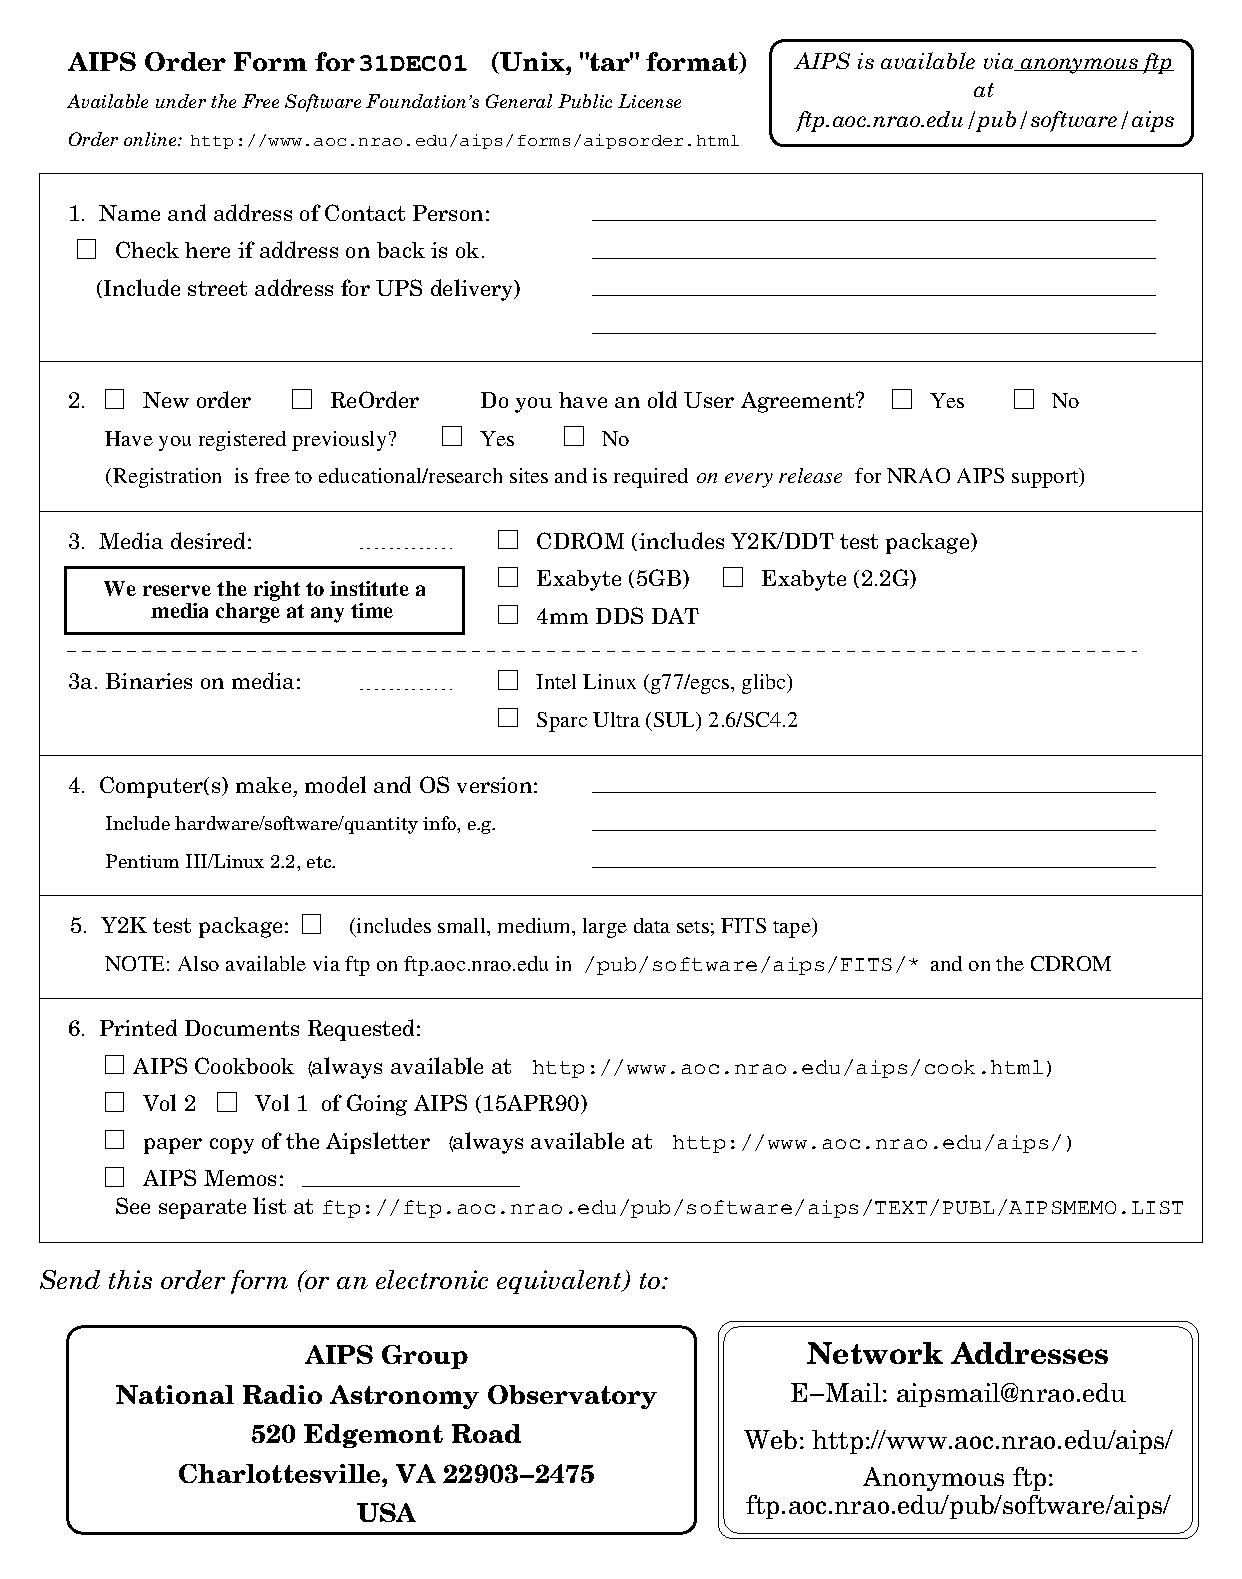
\includegraphics{FIG/AIPSORDER.PS}}}
%\vfill\eject
\vbox to 4.4in{
\vspace{12pt}
%\centerline{\rotatebox{-90}{\resizebox{!}{3.5in}{%
%\includegraphics{FIG/Mandrill.color.plt}}}}
\centerline{\resizebox{!}{3.5in}{\includegraphics{FIG/Mandrill.eps}}}
\vspace{12pt}
\centerline{{\huge \tt \AIPRELEASE}}
\vspace{12pt}
\vfill}
\phantom{...}
\centerline{\resizebox{!}{!}{\includegraphics{FIG/AIPSLETS.PS}}}

\end{document}
